\documentclass{standalone}

\usepackage{tikz}

\usetikzlibrary{calc}

\begin{document}
  %noformat{
  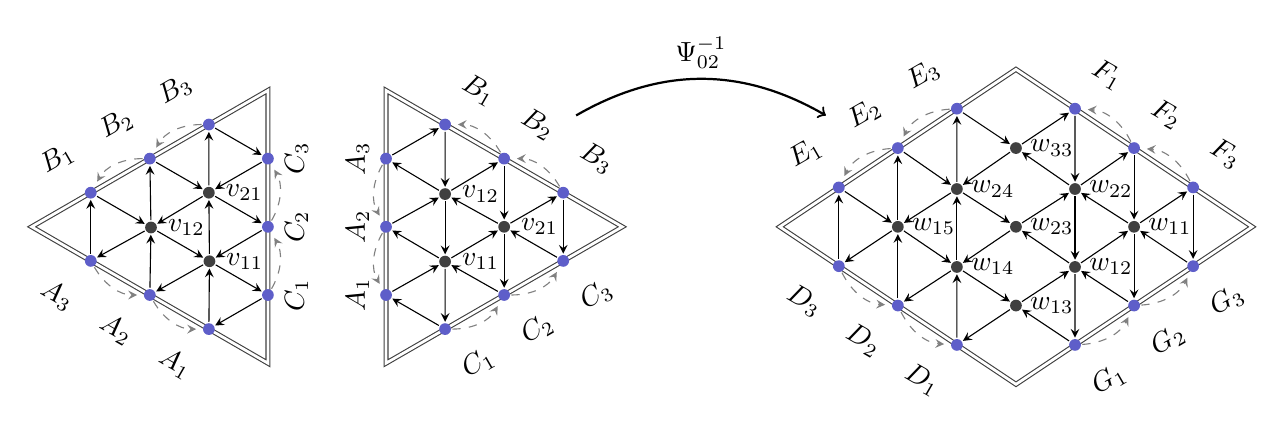
\begin{tikzpicture}
    \tikzstyle{v1} = [circle, outer sep=0.5pt, fill, inner sep=1.5pt]
    \tikzstyle{unf} = [color=darkgray]
    \tikzstyle{frz} = [color=blue!60!darkgray!70]
    \tikzstyle{e} = [->, >={stealth}]
    \tikzstyle{b} = [fill, fill opacity=0.0, circle, outer sep=0.5pt, inner sep=1.5pt]
    \tikzstyle{te} = [color=darkgray, double distance=1pt]
    \tikzstyle{h} = [dashed, color=gray, ->, >={stealth}]
    \tikzstyle{ll} = [color=blue!60!darkgray!70]

    \begin{scope}[shift={(-0.5,0)}]
      \coordinate (l_0) at (-60:2.0);
      \coordinate (l_1) at (180:2.0);
      \coordinate (l_2) at ( 60:2.0);

      \draw[te] (l_0) -- (l_1) -- (l_2) -- cycle;

      \node[v1, frz, label={240:{\rotatebox{330    }{$A_1$}}}] (A1) at ($ (l_0)!0.25!(l_1) $) {};
      \node[v1, frz, label={240:{\rotatebox{330    }{$A_2$}}}] (A2) at ($ (l_0)!0.50!(l_1) $) {};
      \node[v1, frz, label={240:{\rotatebox{330    }{$A_3$}}}] (A3) at ($ (l_0)!0.75!(l_1) $) {};

      % As of writing, rotatebox{90}{} will crash on at least one machine
      \node[v1, frz, label={  0:{\rotatebox{ 90.001}{$C_1$}}}] (C1) at ($ (l_2)!0.75!(l_0) $) {};
      \node[v1, frz, label={  0:{\rotatebox{ 90.001}{$C_2$}}}] (C2) at ($ (l_2)!0.50!(l_0) $) {};
      \node[v1, frz, label={  0:{\rotatebox{ 90.001}{$C_3$}}}] (C3) at ($ (l_2)!0.25!(l_0) $) {};

      \node[v1, frz, label={120:{\rotatebox{ 30    }{$B_1$}}}] (B1) at ($ (l_1)!0.25!(l_2) $) {};
      \node[v1, frz, label={120:{\rotatebox{ 30    }{$B_2$}}}] (B2) at ($ (l_1)!0.50!(l_2) $) {};
      \node[v1, frz, label={120:{\rotatebox{ 30    }{$B_3$}}}] (B3) at ($ (l_1)!0.75!(l_2) $) {};

      \node[v1, unf, label={[label distance=0pt]0:$v_{11}$}] (v11) at ($ (C1)!0.33!(B1) $) {};
      \node[v1, unf, label={[label distance=0pt]0:$v_{12}$}] (v12) at ($ (C1)!0.66!(B1) $) {};
      \node[v1, unf, label={[label distance=0pt]0:$v_{21}$}] (v21) at ($ (C2)!0.50!(B2) $) {};

      \draw[e] (v11) --  (C1);
      \draw[e] (v12) -- (v11);
      \draw[e]  (B1) -- (v12);
      \draw[e] (v21) --  (C2);
      \draw[e]  (B2) -- (v21);
      \draw[e]  (B3) --  (C3);

      \draw[e] (v21) --  (B3);
      \draw[e] (v11) -- (v21);
      \draw[e]  (A1) -- (v11);
      \draw[e] (v12) --  (B2);
      \draw[e]  (A2) -- (v12);
      \draw[e]  (A3) --  (B1);

      \draw[e] (v12) --  (A3);
      \draw[e] (v21) -- (v12);
      \draw[e]  (C3) -- (v21);
      \draw[e] (v11) --  (A2);
      \draw[e]  (C2) -- (v11);
      \draw[e]  (C1) --  (A1);

      \draw[h,-{>[sep=2pt]}] (A3) to[bend right=30] (A2);
      \draw[h,-{>[sep=2pt]}] (A2) to[bend right=30] (A1);
      \draw[h,-{>[sep=2pt]}] (B3) to[bend right=30] (B2);
      \draw[h,-{>[sep=2pt]}] (B2) to[bend right=30] (B1);
      \draw[h,-{>[sep=2pt]}] (C1) to[bend right=30] (C2);
      \draw[h,-{>[sep=2pt]}] (C2) to[bend right=30] (C3);
    \end{scope}

    \begin{scope}[shift={(3,0)}]
      \coordinate (r_0) at (240:2.0);
      \coordinate (r_1) at (120:2.0);
      \coordinate (r_2) at (  0:2.0);

      \draw[te] (r_0) -- (r_1) -- (r_2) -- cycle;

      \node[v1, frz, label={180:{\rotatebox{ 90.001}{$A_1$}}}] (A1) at ($ (r_0)!0.25!(r_1) $) {};
      \node[v1, frz, label={180:{\rotatebox{ 90.001}{$A_2$}}}] (A2) at ($ (r_0)!0.50!(r_1) $) {};
      \node[v1, frz, label={180:{\rotatebox{ 90.001}{$A_3$}}}] (A3) at ($ (r_0)!0.75!(r_1) $) {};

      \node[v1, frz, label={-60:{\rotatebox{ 30    }{$C_1$}}}] (C1) at ($ (r_2)!0.75!(r_0) $) {};
      \node[v1, frz, label={-60:{\rotatebox{ 30    }{$C_2$}}}] (C2) at ($ (r_2)!0.50!(r_0) $) {};
      \node[v1, frz, label={-60:{\rotatebox{ 30    }{$C_3$}}}] (C3) at ($ (r_2)!0.25!(r_0) $) {};

      \node[v1, frz, label={ 60:{\rotatebox{-30    }{$B_1$}}}] (B1) at ($ (r_1)!0.25!(r_2) $) {};
      \node[v1, frz, label={ 60:{\rotatebox{-30    }{$B_2$}}}] (B2) at ($ (r_1)!0.50!(r_2) $) {};
      \node[v1, frz, label={ 60:{\rotatebox{-30    }{$B_3$}}}] (B3) at ($ (r_1)!0.75!(r_2) $) {};

      \node[v1, unf, label={[label distance=0pt]0:$v_{11}$}] (v11) at ($ (C1)!0.33!(B1) $) {};
      \node[v1, unf, label={[label distance=0pt]0:$v_{12}$}] (v12) at ($ (C1)!0.66!(B1) $) {};
      \node[v1, unf, label={[label distance=0pt]0:$v_{21}$}] (v21) at ($ (C2)!0.50!(B2) $) {};

      \draw[e] (v11) --  (C1);
      \draw[e] (v12) -- (v11);
      \draw[e]  (B1) -- (v12);
      \draw[e] (v21) --  (C2);
      \draw[e]  (B2) -- (v21);
      \draw[e]  (B3) --  (C3);

      \draw[e] (v21) --  (B3);
      \draw[e] (v11) -- (v21);
      \draw[e]  (A1) -- (v11);
      \draw[e] (v12) --  (B2);
      \draw[e]  (A2) -- (v12);
      \draw[e]  (A3) --  (B1);

      \draw[e] (v12) --  (A3);
      \draw[e] (v21) -- (v12);
      \draw[e]  (C3) -- (v21);
      \draw[e] (v11) --  (A2);
      \draw[e]  (C2) -- (v11);
      \draw[e]  (C1) --  (A1);

      \draw[h,-{>[sep=2pt]}] (A3) to[bend right=30] (A2);
      \draw[h,-{>[sep=2pt]}] (A2) to[bend right=30] (A1);
      \draw[h,-{>[sep=2pt]}] (B3) to[bend right=30] (B2);
      \draw[h,-{>[sep=2pt]}] (B2) to[bend right=30] (B1);
      \draw[h,-{>[sep=2pt]}] (C1) to[bend right=30] (C2);
      \draw[h,-{>[sep=2pt]}] (C2) to[bend right=30] (C3);
    \end{scope}

    \begin{scope}[shift={(10,0)}]
      \coordinate (q_0) at (270:2);
      \coordinate (q_1) at (180:3);
      \coordinate (q_2) at ( 90:2);
      \coordinate (q_3) at (  0:3);

      \draw[te] (q_0) -- (q_1) -- (q_2) -- (q_3) -- cycle;

      \node[v1, frz, label={240:{\rotatebox{330}{$D_1$}}}] (D1) at ($ (q_0)!0.25!(q_1) $) {};
      \node[v1, frz, label={240:{\rotatebox{330}{$D_2$}}}] (D2) at ($ (q_0)!0.50!(q_1) $) {};
      \node[v1, frz, label={240:{\rotatebox{330}{$D_3$}}}] (D3) at ($ (q_0)!0.75!(q_1) $) {};

      \node[v1, frz, label={120:{\rotatebox{ 30}{$E_1$}}}] (E1) at ($ (q_1)!0.25!(q_2) $) {};
      \node[v1, frz, label={120:{\rotatebox{ 30}{$E_2$}}}] (E2) at ($ (q_1)!0.50!(q_2) $) {};
      \node[v1, frz, label={120:{\rotatebox{ 30}{$E_3$}}}] (E3) at ($ (q_1)!0.75!(q_2) $) {};

      \node[v1, frz, label={ 60:{\rotatebox{-30}{$F_1$}}}] (F1) at ($ (q_2)!0.25!(q_3) $) {};
      \node[v1, frz, label={ 60:{\rotatebox{-30}{$F_2$}}}] (F2) at ($ (q_2)!0.50!(q_3) $) {};
      \node[v1, frz, label={ 60:{\rotatebox{-30}{$F_3$}}}] (F3) at ($ (q_2)!0.75!(q_3) $) {};

      \node[v1, frz, label={-60:{\rotatebox{ 30}{$G_1$}}}] (G1) at ($ (q_0)!0.25!(q_3) $) {};
      \node[v1, frz, label={-60:{\rotatebox{ 30}{$G_2$}}}] (G2) at ($ (q_0)!0.50!(q_3) $) {};
      \node[v1, frz, label={-60:{\rotatebox{ 30}{$G_3$}}}] (G3) at ($ (q_0)!0.75!(q_3) $) {};

      \node[v1, unf, label={[label distance=-1pt]0:$w_{15}$}] (w15) at ($ (D2)!0.50!(E2) $) {};
      \node[v1, unf, label={[label distance=-1pt]0:$w_{14}$}] (w14) at ($ (D1)!0.33!(E3) $) {};
      \node[v1, unf, label={[label distance=-1pt]0:$w_{24}$}] (w24) at ($ (D1)!0.66!(E3) $) {};

      \node[v1, unf, label={[label distance=-1pt]0:$w_{13}$}] (w13) at ($ (q_0)!0.25!(q_2) $) {};
      \node[v1, unf, label={[label distance=-1pt]0:$w_{23}$}] (w23) at ($ (q_0)!0.50!(q_2) $) {};
      \node[v1, unf, label={[label distance=-1pt]0:$w_{33}$}] (w33) at ($ (q_0)!0.75!(q_2) $) {};

      \node[v1, unf, label={[label distance=-1pt]0:$w_{11}$}] (w11) at ($ (G2)!0.50!(F2) $) {};
      \node[v1, unf, label={[label distance=-1pt]0:$w_{12}$}] (w12) at ($ (G1)!0.33!(F1) $) {};
      \node[v1, unf, label={[label distance=-1pt]0:$w_{22}$}] (w22) at ($ (G1)!0.66!(F1) $) {};


      %\draw[e]  (F3) --  (G3);
      %\draw[e]  (F2) -- (w11);
      %\draw[e] (w11) --  (G2);
      %\draw[e]  (F1) -- (w22);
      %\draw[e] (w22) -- (w12);
      %\draw[e] (w12) --  (G1);
      %\draw[e] (w24) --  (E3);
      %\draw[e] (w14) -- (w24);
      %\draw[e]  (D1) -- (w14);
      %\draw[e] (w15) --  (E2);
      %\draw[e]  (D2) -- (w15);
      %\draw[e]  (D3) --  (E1);

      \draw[e] (w14) -- (w13);
      \draw[e] (w15) -- (w14);
      \draw[e]  (E1) -- (w15);
      \draw[e] (w24) -- (w23);
      \draw[e]  (E2) -- (w24);
      \draw[e]  (E3) -- (w33);

      \draw[e] (w24) --  (E3);
      \draw[e] (w14) -- (w24);
      \draw[e]  (D1) -- (w14);
      \draw[e] (w15) --  (E2);
      \draw[e]  (D2) -- (w15);
      \draw[e]  (D3) --  (E1);

      \draw[e] (w15) --  (D3);
      \draw[e] (w24) -- (w15);
      \draw[e] (w33) -- (w24);
      \draw[e] (w14) --  (D2);
      \draw[e] (w23) -- (w14);
      \draw[e] (w13) --  (D1);

      \draw[e] (w12) --  (G1);
      \draw[e] (w22) -- (w12);
      \draw[e]  (F1) -- (w22);
      \draw[e] (w11) --  (G2);
      \draw[e]  (F2) -- (w11);
      \draw[e]  (F3) --  (G3);

      \draw[e] (w11) --  (F3);
      \draw[e] (w12) -- (w11);
      \draw[e] (w13) -- (w12);
      \draw[e] (w22) --  (F2);
      \draw[e] (w23) -- (w22);
      \draw[e] (w33) --  (F1);

      \draw[e] (w22) -- (w33);
      \draw[e] (w11) -- (w22);
      \draw[e]  (G3) -- (w11);
      \draw[e] (w12) -- (w23);
      \draw[e]  (G2) -- (w12);
      \draw[e]  (G1) -- (w13);

      \draw[h,-{>[sep=2pt]}] (D3) to[bend right=30] (D2);
      \draw[h,-{>[sep=2pt]}] (D2) to[bend right=30] (D1);
      \draw[h,-{>[sep=2pt]}] (E3) to[bend right=30] (E2);
      \draw[h,-{>[sep=2pt]}] (E2) to[bend right=30] (E1);
      \draw[h,-{>[sep=2pt]}] (F3) to[bend right=30] (F2);
      \draw[h,-{>[sep=2pt]}] (F2) to[bend right=30] (F1);
      \draw[h,-{>[sep=2pt]}] (G1) to[bend right=30] (G2);
      \draw[h,-{>[sep=2pt]}] (G2) to[bend right=30] (G3);
    \end{scope}

    \draw[->, thick]
        ($ (3,0) + ( 45:2) $)
        to[bend left] node[midway, above] (t01) {$\Psi_{02}^{-1}$}
        ($ (9,0) + (135:2) $);

  \end{tikzpicture}
  %}noformat
\end{document}
